\documentclass{beamer}

\mode<presentation>
{
  \usetheme{CambridgeUS}
  \setbeamercovered{transparent}
}

\usepackage[T1]{fontenc}
\usepackage[utf8]{inputenc}
\usepackage[spanish]{babel}
\usepackage{color}
\usepackage{hyperref}
\usepackage{algorithm,algorithmic}
\usepackage{colortbl}
\usepackage{graphicx}

\title[\textbf{Programación 2}]{\textbf{Programación 2}}

\subtitle{Introducción a la Orientación a Objetos}

\author[IF-EG]
{Profesores:\\
  Ismael Figueroa -  \texttt{\small ifigueroap@gmail.com} \\
  \vspace{0.5mm} \\
  Eduardo Godoy - \texttt{\small eduardo.gl@gmail.com}
}

\institute[Universidad de Valparaíso]

\date{}

\begin{document}

\begin{frame}
  \titlepage
\end{frame}

\begin{frame}
  \frametitle{Contenido}
  \tableofcontents%[pausesections]
\end{frame}

\section{Introducción}

\subsection{Antes de comenzar}

\begin{frame}

  \begin{block}{\textquestiondown Qué es la Orientación a Objeto?}
    De manera sintetizada, la orientación a objetos es un \textbf{{\em
        paradigma}} de programación.
  \end{block}

  \begin{block}{\textquestiondown Qué es un paradigma?}
    Un paradigma de programación es un modelo básico de dise\~no y
    desarrollo de soluciones, con directrices específicas, tales como:
    estructura, cohesión, acoplamiento, etc.
  \end{block}
  
  \begin{exampleblock}{En general}
    El Paradigma de Orientación a Objeto es \textbf{una forma} de
    entender un problema, identificando las principales
    \textbf{entidades} que se encuentran en él.
  \end{exampleblock}
\end{frame}

\begin{frame}

  \begin{block}{\textquestiondown Qué es un Lenguaje de Programación?}
    Es la \textbf{herramienta} seleccionada, para dar solución al
    problema detectado.
  \end{block}

  \begin{block}{En relación a los Lenguajes de Programación}
    Se es libre de utilizar la herramienta con la cual se esté más
    habituado. La solución final no cambia.
  \end{block}
  
  \begin{exampleblock}{Corolario}
    El Paradigma de Orientación a Objetos no está dado por un solo
    lenguaje específico, si no por la forma de entender y solucionar
    problemas. Hay lenguajes que ayudan más o menos a trabajar con esa
    forma.
  \end{exampleblock}
\end{frame}

\subsection{Tipos de Paradigma}

\begin{frame}

  \begin{itemize}
  \item \textbf{Procedural o imperativo:}
    \begin{itemize}
    \item Se describe como una secuencia instrucciones o comandos
      que cambian el estado de un programa. El código máquina en
      general está basado en el paradigma imperativo.
    \end{itemize}
    
  \item \textbf{Declarativo:}
    \begin{itemize}
    \item Se basa en el \textbf{qué} hacer y no en el cómo. Está
      basado en el desarrollo de programas especificando o
      \textbf{{\em declarando}} un conjunto de condiciones,
      proposiciones, afirmaciones, restricciones, ecuaciones o
      transformaciones que describen el problema y detallan su
      solución.
    \end{itemize}
    
  \item \textbf{Lógico:}
    \begin{itemize}
    \item Se basa en la definición de reglas lógicas para luego, a
      través de un motor de inferencias lógicas, responder preguntas
      planteadas al sistema y así resolver problemas.
    \end{itemize}
  \end{itemize}

\end{frame}

\begin{frame}
  
  \begin{itemize}
  \item \textbf{Estructurado:}
    \begin{itemize}
    \item La programación se divide en \textbf{bloques}
      (procedimientos y funciones) que pueden o no comunicarse entre
      sí. Además la programación se controla con secuencia,
      selección e iteración. Su principal ventaja es la
      \emph{estructura clara} lo que entrega una mejor comprensión
      de la programación.
    \end{itemize}
    
  \item \textbf{Funcional:} 
    \begin{itemize}
    \item Concibe a la computación como la evaluación de funciones y
      evita declarar y cambiar datos. En otras palabras, hace
      hincapié en la aplicación de las funciones y composición entre
      ellas.
    \end{itemize}

  \item \textbf{Orientado a Objetos:}
    \begin{itemize}
    \item Utiliza objetos y sus interacciones, para diseñar
      aplicaciones y programas informáticos. Está basado en varias
      técnicas, incluyendo abstracción, encapsulamiento, ocultamiento,
      herencia, polimorfismo, entre otras.
    \end{itemize}
    
  \end{itemize}
\end{frame}

\section{Conceptos}

\subsection{Programación Orientada a Objetos}
\begin{frame}
  \frametitle{¿Qué es la POO?}

  \begin{exampleblock}{}
    \begin{itemize}
    \item[] La \textbf{POO} se basa en la dividir el programa en peque\~nas unidades lógicas de código. A estas peque\~nas unidades lógicas de código se les denomina \textbf{objetos}. Los objetos son unidades independientes que se comunican entre ellos.\\
    \item[] La \textbf{POO} proporciona técnicas con las cuales se
      modela y representa el mundo real (tan fielmente como sea
      posible).
    \end{itemize}
  \end{exampleblock}
\end{frame}

\begin{frame}
  \frametitle{¿Qué es un Objeto?}

  \begin{exampleblock}{}
    \begin{itemize}
    \item[] Cualquier cosa que vemos a nuestro alrededor. Ej: auto.
    \item[] Un objeto, en general, está compuesto por:
      \begin{itemize}
      \item \emph{Características} tales como: marca, modelo, color, etc.
      \item \emph{Comportamiento}, por ejemplo: encender, acelerar, frenar, retroceder, etc.
      \end{itemize}
    \end{itemize}
  \end{exampleblock}
\end{frame}

\begin{frame}
  \frametitle{¿Cómo se caracterizan los objetos?}

  \begin{block}{Características}
    Los objetos tienen un \emph{estado interno} que se representa
    mediante variables conocidas como \emph{atributos}.
  \end{block}

  \begin{block}{Comportamiento}
    Además, el comportamiento de los objetos se programa mediante
    \emph{métodos}, que son funciones o procedimientos que tienen acceso
    directo al estado interno del objeto.
  \end{block}

\end{frame}

\begin{frame}
  \frametitle{Clases e Instancias}

  \begin{itemize}
  \item \textbf{Clases:}    
    \begin{itemize}
    \item[] Modelo para múltiples objetos con características y
      comportamientos similares. Las clases comprenden todas las
      características de una serie particular de objetos. En
      \textbf{POO} se definen clases como un modelo abstracto de un
      objeto. Lo más parecido en C es un struct.
    \end{itemize}
    
  \item \textbf{Instancias de una clase:}
    \begin{itemize}
    \item[] Representación concreta de un objeto. Al definir una clase
      se pueden crear muchas instancias de la misma y cada instancia
      puede tener diferentes características mientras se comporte y
      reconozca como objeto de la clase. En programación estructurada
      sería una \emph{variable}.
    \end{itemize}
    
  \end{itemize}
\end{frame}

\begin{frame}
  \frametitle{Características de un Objeto} 

  \begin{itemize}
  \item \textbf{Atributos:}
    \begin{itemize}
    \item[] Características que diferencian a un objeto de otro y
      determinan la ''\emph{forma}'' de ese objeto.
      
    \item[] Los atributos se definen como \textbf{variables}. De hecho
      podrían, ser vistas como \textbf{variables globales del
        objeto}. Cada instancia de una clase puede tener diferentes
      valores para sus variables, por lo que a cada variable se le
      denomina \textbf{variable de instancia}. La clase define el tipo
      de atributo y cada instancia guarda su propio valor para ese
      atributo.
    \end{itemize}
  \end{itemize}
\end{frame}

\begin{frame}
  \frametitle{Características de un Objeto}

  \begin{itemize}
  \item \textbf{Métodos:}
    \begin{itemize}

    \item[] Comúnmente denominadas \textbf{funciones} o
      \textbf{procedimientos} definidas dentro de una clase, y que
      operan en sus instancias. Los objetos se \textbf{comunican}
      entre sí mediante el uso \textbf{llamadas a de métodos}. Se dice
      que una clase puede \textbf{llamar} al método de otra clase.
      
    \item[] Se pueden definir métodos de instancia (que operan en una
      instancia de la clase) y los métodos de clase que operan sobre
      la clase.
      
    \end{itemize}
  \end{itemize}
\end{frame}

\begin{frame}
  \frametitle{Representación Gráfica}
  \framesubtitle{Clases}

  \begin{itemize}
  \item Una clase se representa como un rectángulo con 3 secciones:
    \begin{enumerate}
    \item El nombre de la clase      
    \item Los nombres y tipos de sus atributos      
    \item Los nombres, parámetros y tipo de retorno de los métodos
    \end{enumerate}
    
  \item Los atributos y métodos pueden ser:
    \begin{itemize}
    \item Públicos: se antepone el signo $+$      
    \item Protegidos: se antepone el signo $\#$      
    \item Privados: se antepone el signo $-$
    \end{itemize}
    Si no aparecen los signos, se asume que el elemento es público
  \end{itemize}

\end{frame}

\begin{frame}
  \frametitle{Representación Gráfica}
  \framesubtitle{Instancias}

  \begin{itemize}
  \item Una instancia se representa también con un rectángulo, pero
    con 2 secciones:
    \begin{enumerate}
    \item El nombre de la instancia y la clase a la que pertenece
    \item Los nombres y valores asociados a los atributos  
    \end{enumerate}
  \end{itemize}    

    Los métodos no se muestran en la instancia, porque están
    contenidos siempre en la clase correspondiente.

  \end{frame}

  \begin{frame}
    \frametitle{Representación Gráfica}
    \framesubtitle{Clases e Instancias}
    
    \begin{center}
      \begin{figure}[!t]
        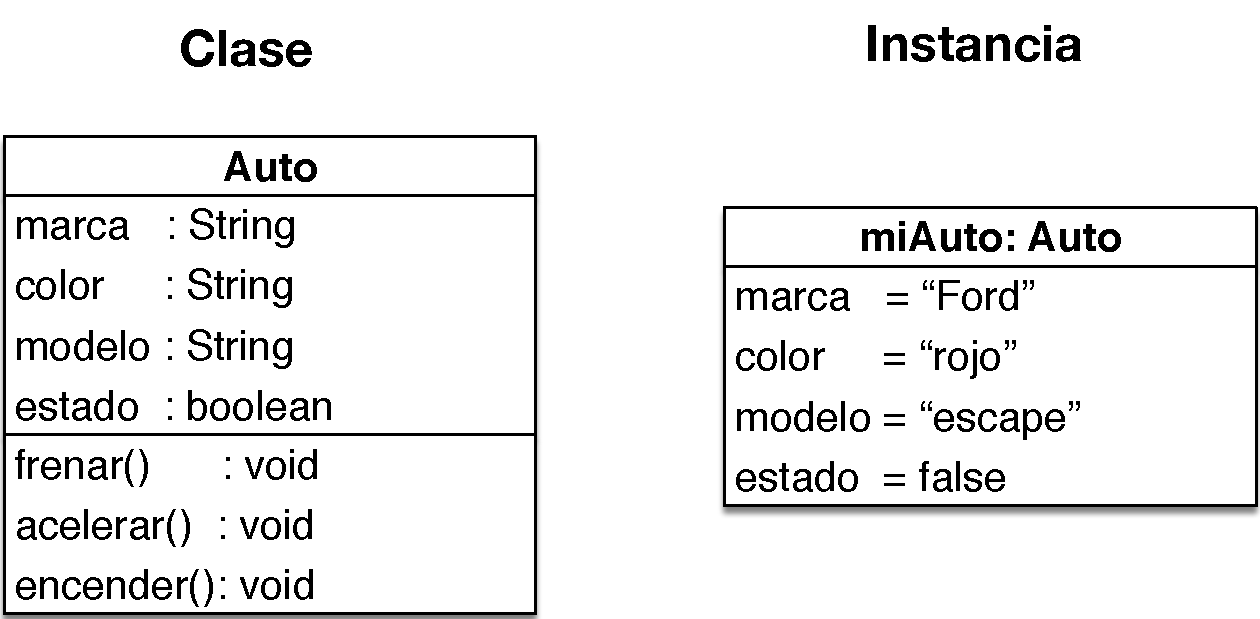
\includegraphics[scale=.4]{images/uml_clase_instancia}
      \end{center}
    \end{figure}  

  \end{frame}

  \subsection{Elementos de POO}

  \begin{frame}
    \frametitle{Abstracción}

    \begin{itemize}
    \item Capacidad de analizar y representar las características
      esenciales de fenómenos complejos.
      
    \item Una clase es una abstracción o una entidad esencial del
      problema o la solución.
      
    \item Ejemplo: 
      \begin{itemize}
      \item[] Qué características tienen de los autos?
      \item[] Qué comportamiento tienen los autos?
      \end{itemize}
      
    \item En la \textbf{POO} el concepto de clase es la representación
      y el mecanismo por el cual se gestionan las abstracciones.
    \end{itemize}

  \end{frame}


  \begin{frame}
    \frametitle{Encapsulamiento}

    \begin{itemize}
      
    \item Técnica para proteger y ocultar el estado interno y el {\em conocimiento} de una entidad.

    \item En el paradigma de la orientación a objetos, la clase/objeto
      es la unidad fundamental de encapsulamiento.
      
    \item En la POO la utilidad del encapsulamiento va por la
      facilidad de manejar la complejidad, ya que tendremos clases
      (como cajas negras) donde sólo se conoce el comportamiento pero
      no los detalles internos.
      
    \end{itemize}
  \end{frame}				


  \begin{frame}
    \frametitle{Ocultamiento de Información}

    \begin{itemize}
      
    \item Es la capacidad de ocultar los detalles internos del
      comportamiento de una clase y exponer sólo los detalles que sean
      necesarios para el resto del sistema.
      
    \item Cada tipo de objeto expone una \textbf{interfaz} que
      especifica como pueden interactuar con los objetos de la clase.
      
    \item En la \textbf{POO} el objeto tiene, al menos, dos vistas:
      \begin{itemize}
        
      \item[] Restringir el uso de la clase, pues habrá cierto
        comportamiento \textbf{privado} que no podrá ser accedido por
        otras clases.
        
      \item[] Controlar el uso de la clase, pues se darán ciertos
        mecanismos para modificar el estado de una clase.
        
      \end{itemize}      
    \end{itemize}
  \end{frame}

  \begin{frame}
    \frametitle{Herencia}

    \begin{itemize}
    \item Organización jerárquica de clases.
      
    \item Cada clase tiene una superclase y puede tener una o más
      subclases.
      
    \item Las subclases heredan todos los atributos y métodos de la
      superclase, esto significa que las subclases incorporan a sus
      atributos y métodos propios, los atributos y métodos heredados
      de la superclase.
      
    \item En la parte superior de la jerarquía de clases, está la
      clase \textbf{Object}. Todas las clases heredan de esta
      superclase y cada clase hacia abajo agrega más información.

    \item Gráficamente, una subclase apunta con una flecha blanca
      hacia su superclase.
    \end{itemize}

  \end{frame}

  \begin{frame}
    \frametitle{Herencia}
    \framesubtitle{Ejemplo Jerarquía de Herencia}
    \begin{center}
      \begin{figure}[!t]
        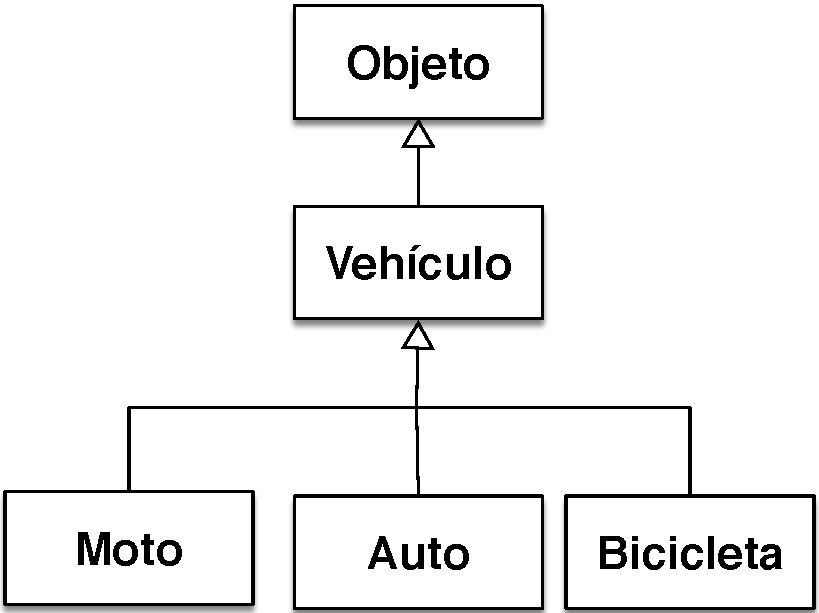
\includegraphics[scale=.6]{images/jerarquia_1}
      \end{figure}
    \end{center}
  \end{frame}

  \begin{frame}
    \frametitle{Herencia}
    \framesubtitle{Ejemplo Jerarquía de Herencia}
    \begin{center}
      \begin{figure}[!t]
        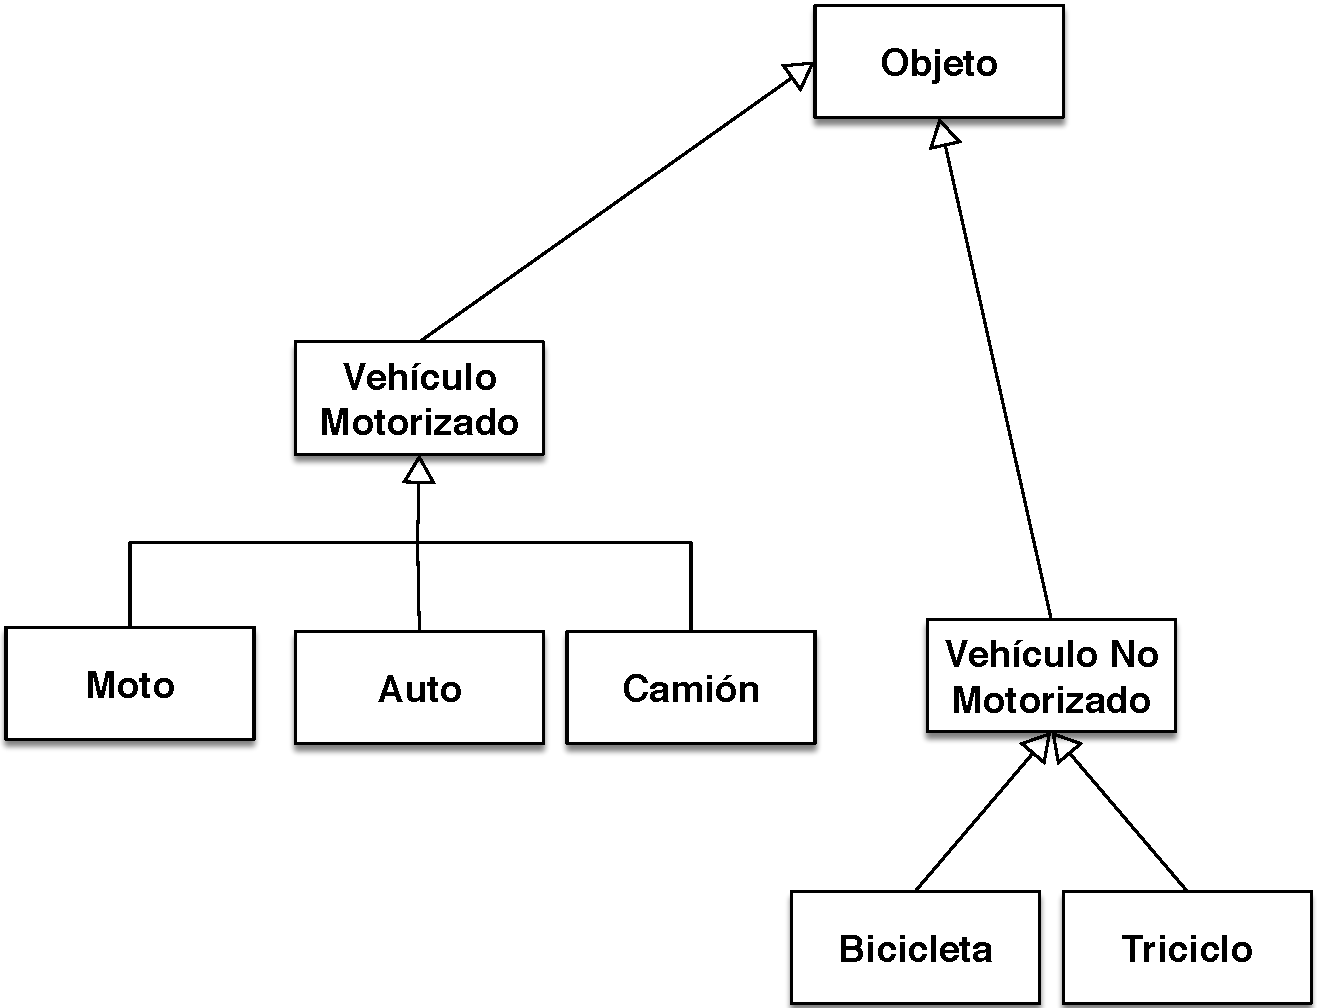
\includegraphics[scale=.4]{images/jerarquia_2}
      \end{figure}
    \end{center}
  \end{frame}

  \begin{frame}
    \frametitle{Polimorfismo}
    \begin{itemize}
      
    \item Literalmente, \textbf{Poli (muchos/as) - Morphus(formas)}.
      
    \item La interfaz de un método, es decir su nombre, parámetros y tipo de
      retorno pueden especificarse de manera general.
      
    \item Cada clase que implementa el método, lo hace de manera
      independiente y particular---pero se sigue teniendo el mismo
      nombre.
      
    \item Se pueden implementar distintas funcionalidades, que dependen
      de las clases involucradas, pero que se programan de manera
      genérica con el mismo nombre.
      
    \item \textbf{Beneficios:} Código más genérico. Solo basta saber que
      un objeto/clase implementa una interfaz para poder
      utilizarlo. Maximiza la calidad de reuso, la extensibilidad, y la
      inter-operabilidad entre distintas implementaciones.
      
    \item \textbf{Ejemplo:}
      \begin{itemize}
        
      \item La interfaz List define listas con cantidad arbitraria de
        elementos. Existen diversas implementaciones.
        
      \item Todas las implementaciones definen el método add para
        agregar elementos
        
      \item Un programa que usa listas, no necesita saber cuál de las
        implementaciones está usando      
        
      \end{itemize}
    \end{itemize}
  \end{frame}

  \begin{frame}
    \frametitle{Envío de Mensajes}

    \begin{itemize}
    \item \textbf{Envío de mensajes:}
      \begin{itemize}
      \item Un objeto es inútil si está aislado.
      \item Los objetos de un programa interactúan y se comunican entre ellos por medio de \textbf{mensajes}.
      \item Cuando un \textbf{objeto A} quiere que un \textbf{objeto B} ejecute una de sus funciones (métodos del objeto B), el objeto A \textbf{envía un mensaje} al objeto B. Los mensajes son invocaciones a los métodos de los objetos. 
      \item Ejemplo: si objeto \emph{miAuto} debe acelerar.
        \begin{itemize}
        \item[] El objeto al cual se manda el mensaje (miAuto).
        \item[] El método que debe ejecutar (acelerar()).
        \item[] Los parámetros que necesita ese método (10 km/h).
        \end{itemize}
      \item Estas tres partes del mensaje (objeto destinatario, método y parámetros) son suficiente información para que el objeto que recibe el mensaje, ejecute el método.
      \end{itemize}
    \end{itemize}
  \end{frame}      

  \begin{frame}
    \frametitle{Preguntas}

    \hspace{4cm}\huge{¿ Preguntas ?}
    
  \end{frame}

\end{document}

\usetheme{default}
\usetheme{JuanLesPins}
\usetheme{Goettingen}
\usetheme{Szeged}
\usetheme{Warsaw}

\usecolortheme{crane}

\usefonttheme{serif}
\usefonttheme{structuresmallcapsserif}